\documentclass {jsarticle}
\usepackage[dvipdfmx]{graphicx}
\usepackage{float}
\usepackage{multicol}
\usepackage{listings,jlisting}
\renewcommand{\lstlistingname}{リスト}
\lstset{
	language=java,%
	basicstyle=\scriptsize,%
	numbersep=5pt,%
	breaklines=true,%
	breakindent=5pt,%
	frame=single,%
	tabsize=2,%
	numbers=left,%
	numberstyle=\tiny,%
	showstringspaces=false%
	}%
\setlength{\columnsep}{20pt}
\setlength{\columnwidth}{200cm}

\begin{document}

\title{知能システム前期末レポート}
\author{15422 篠田拓樹}
\date{\today}
\maketitle
%-----------------------------------------
\newpage
\section{XORを学習するニューラルネットワーク}
  XORを学習するニューラルネットワークを作成した.
リスト\ref{sampleBP.c}に示すプログラムを用いて
実行を行った.

XORの各入力に対して学習がうまくいっていることを
確認した.

また,拡張として行列演算によって前向き,後ろ向き
の計算を行うリスト\ref{newral.py}のプログラム
も作成した.
なお,リスト\ref{sampleBP.c}と同じ重みを用いて学習を
行い,結果が同じになることを確認している.
同様に学習がうまくいっていることを確認した.

学習過程の誤差の変化を図\ref{error-1}に示す.

\begin{figure}[htb]
  \centering
  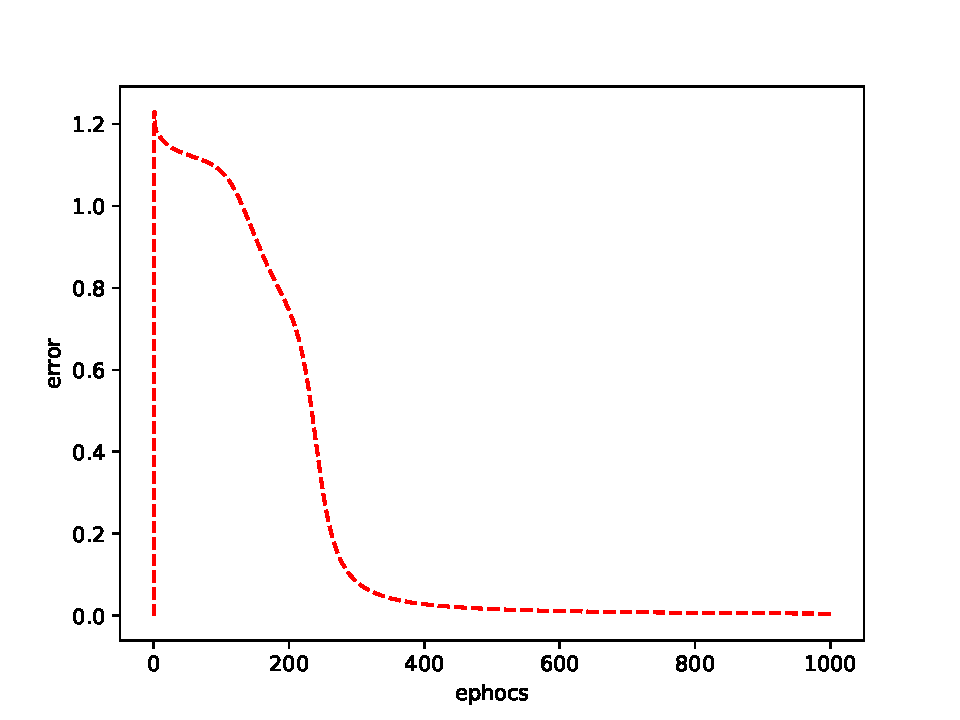
\includegraphics[scale=0.5]{img/error1.pdf}
  \caption{XOR学習時の誤差変化}
  \label{error-1}
\end{figure}

%-----------------------------------------
\section{魚を識別するニューラルネットワーク}
  \input{files/}
%------------------------------------------
\newpage
\section{プログラムリスト}
\begin{multicols}{2}
\lstinputlisting[caption=sampleBP.c,label=sampleBP.c]
{../sample/sampleBP.c}
\lstinputlisting[caption=newral.py,label=newral.py]
{../newral.py}
\end{multicols}

\end{document}
